%%{ DOC HEAD

\pdfoutput=1
\documentclass[a4paper,11pt,titlepage,twoside]{book}

\usepackage[english]{babel}
\usepackage[utf8]{inputenc}
\usepackage{csquotes}

\usepackage{amsmath,amsfonts,amssymb,bm}
\usepackage{nicefrac}

\usepackage{algorithm,algpseudocode}
\usepackage[title,titletoc]{appendix}
\usepackage{latexsym}
\usepackage{a4wide}
\usepackage{color}
\usepackage{indentfirst}
\usepackage{graphicx}       %%% graphics for dvips
\usepackage{fancyhdr,lastpage}
\usepackage{longtable}
\usepackage{pifont}
\usepackage{makeidx}
\usepackage{multirow}
\usepackage{dcolumn}
\usepackage{epstopdf}
\usepackage{url}
\usepackage{listings}
\usepackage{relsize}
\usepackage{pdfpages}
\usepackage{url}
\usepackage{lipsum}
\usepackage{isotope}
\usepackage{verbatim}
\usepackage{xcolor}
\usepackage{tcolorbox}
\usepackage[]{hyperref}

\usepackage{subfig} % subfloat
\usepackage[export]{adjustbox}

\hyphenation{}

%%{ tikz

\usepackage{tikz}
\usepackage{pgfplots}
\pgfplotsset{compat=1.14}
\usetikzlibrary{backgrounds,arrows,automata,shapes,positioning,calc,through,spy}
\pgfdeclarelayer{background}
\pgfdeclarelayer{foreground}
\pgfsetlayers{background,main,foreground}

\tikzset{
    imgletter/.style={
      rectangle,
      inner sep=2pt,
      rounded corners=.1em,
      text=black,
      minimum height=1em,
      text centered,
      fill=white,
      fill opacity=1.0,
      text opacity=1,
      anchor=south west,
  },
}

%%}

%%{ include paper box

% \newcommand{\includepaper}[1]{\includepdf[scale=0.85,pages=-,pagecommand={\thispagestyle{plain}}]{./papers_to_include_pdf/#1}}
\newcommand{\includepaper}[1]{\conditionalClearPage \fullciteinbox{#1}{Here will be the pdf of the paper}}
% \newcommand{\includepaper}[1]{\fullciteinbox{#1}{Here will be the pdf of the paper}}

%%}

%%{ fullcite box

\definecolor{light-gray}{gray}{0.95}
\newcommand{\fullciteinbox}[2]{%

\DeclareCiteCommand{\fullcite}
{\usebibmacro{prenote}}
{\clearfield{addendum}%
  \usedriver
  {\defcounter{minnames}{6}%
  \defcounter{maxnames}{6}}
{\thefield{entrytype}}}
{\multicitedelim}
{\usebibmacro{postnote}}

%\vspace{3em}%
%\raisebox{3em}[3em][3em]{%
% \vspace{-0.2em}
\begin{tcolorbox}[width=\textwidth,colback={light-gray},title={}]%
\ifx&#2&
\else
  \textbf{#2}:\\\\
\fi
\begin{minipage}[t]{0.07\linewidth}%
\raggedright%
\cite{#1}%
\end{minipage}%
\begin{minipage}[t]{0.93\linewidth}%
\fullcite{#1}%
\end{minipage}%
\end{tcolorbox}%
%}%
% \vspace{-0.5em}
}%

%%}

%%{ acronym

\usepackage[nolist,nohyperlinks]{acronym}
\acrodef{GPS}[GPS]{Global Positioning System}
\acrodef{SLAM}[SLAM]{Simultaneous Localization And Mapping}
\acrodef{SLAMs}[SLAMs]{Simultaneous Localization And Mapping systems}
\acrodef{GPS}[GPS]{Global Positioning System}
\acrodef{RTK}[RTK]{Real-time Kinematics}
\acrodef{GNSS}[GNSS]{Global Navigation Satellite System}
\acrodef{ROS}[ROS]{Robot Operating System}
\acrodef{API}[API]{Application Programming Interface}
\acrodef{UAV}[UAV]{Unmanned Aerial Vehicle}
\acrodef{MAV}[MAV]{Micro Aerial Vehicle}
\acrodef{UGV}[UGV]{Unmanned Ground Vehicle}
\acrodef{UV}[UV]{Ultra-Violet}
\acrodef{LED}[LED]{Light-emitting Diode}
\acrodef{MBZIRC}[MBZIRC]{Mohamed Bin Zayed International Robotics Challenge}
\acrodef{DARPA}[DARPA]{Defense Advanced Research Projects Agency}
\acrodef{IMU}[IMU]{Inertial Measurement Unit}
\acrodef{LTI}[LTI]{Linear time-invariant}
\acrodef{MPC}[MPC]{Model Predictive Control}
\acrodef{UVDAR}[UVDAR]{Ultra-Violet Direction And Ranging}
\acrodef{DOF}[DOF]{degree-of-freedom}
\acrodef{DOFs}[DOFs]{degrees-of-freedom}
\acrodef{LiDAR}[LiDAR]{Light Detection and Ranging}
\acrodef{ESC}[ESC]{Electronic Speed Controller}
\acrodef{LKF}[LKF]{Linear Kalman Filter}
\acrodef{UKF}[UKF]{Unscented Kalman Filter}
\acrodef{EKF}[EKF]{Extended Kalman Filter}
\acrodef{RAS}[RAS]{Robotics and Automation Society}
\acrodef{IEEE}[IEEE]{Institute of Electrical and Electronics Engineers}
\acrodef{MRS}[MRS]{Multi-robot Systems Group}
\acrodef{FOV}[FOV]{Field of View}
\acrodef{CdTe}[CdTe]{Cadmium Telluride}
\acrodef{FDNPP}[FDNPP]{Fukushima Daiichi Nuclear Power Plant}

%%}

%%{ siunitx

\usepackage{siunitx}
\DeclareSIUnit \parsec {pc}
\DeclareSIUnit \electronvolt {eV}
\DeclareSIUnit \pixel {px}
\DeclareSIUnit \arcmin {arcmin}
\DeclareSIUnit \erg {erg}
\DeclareSIUnit \joul {J}

%%}

%%{ change formatting of lists

\usepackage{enumitem}
\setlist{nosep}
% \setlist{noitemsep}
% how to format particular lists?
% \begin{itemize}[topsep=8pt,itemsep=4pt,partopsep=4pt, parsep=4pt]

%%}

%%{ change spacing of the table of contents

% \usepackage{tocloft}
% \renewcommand\cftchapafterpnum{\vskip5pt}
% \renewcommand\cftsecafterpnum{\vskip5pt}

%%}

%%{ change formatting of a chapter

\usepackage{titlesec}
\titleformat{\chapter}[block]
{\normalfont\huge\bfseries}{Chapter \thechapter\\\vspace{0.1em}\\}{1em}{\Huge}
% {?}{before}{after}
\titlespacing*{\chapter}{0pt}{-1em}{2em}

%%}

%%{ BIBLATEX

\usepackage[backend=bibtex,defernumbers=true,style=ieee,sorting=ydnt,sortcites=true]{biblatex}

\renewcommand*{\bibfont}{\Font}

% \newcounter{mycounter}
% \setcounter{mycounter}{0}
% \newcounter{unrelatedcount}
% \setcounter{unrelatedcount}{0}
% \newcounter{totalcounter}
% \setcounter{totalcounter}{0}

% % Print labelnumbers with suffixes, adjust secondary labelnumber 1/2 (start new numbering of my publications)
% \makeatletter
% \AtDataInput{%
%   \ifkeyword{mine}
%   {
%     \addtocounter{mycounter}{1}
%   }
%   {}
%   \addtocounter{totalcounter}{1}
% }
% \makeatother

% Print labelnumbers with suffixes, adjust secondary labelnumber 2/2
\DeclareFieldFormat{labelnumber}{%
  \ifkeyword{mine}
    {\ifkeyword{core}
      {{\number\numexpr#1}c}%
      {{\number\numexpr#1}a}%
    }%
    {#1}%
}

% {{\number\numexpr#1-\value{bbx:primcount}}a}

\addbibresource{main.bib}

\defbibenvironment{favoritebib}
{\itemize}
{\enditemize}
{\item}

%%}

%%{ CUSTOM MACROS

%%%%%%%%%%%%%%% changemargin environment begin %%%%%%%%%%%%%%%%%%%%%%%%%
\def\changemargin#1#2{\list{}{\rightmargin#2\leftmargin#1}\item[]}
\let\endchangemargin=\endlist
%%%%%%%%%%%%%%% changemargin environment end %%%%%%%%%%%%%%%%%%%%%%%%%

\newcommand{\strong}[1]{\textbf{#1}}
\newcommand{\coord}[1]{\textbf{#1}}
\newcommand{\norm}[1]{\left\lvert#1\right\rvert}
\newcommand{\m}[1]{\ensuremath{\mathbf{#1}}}
\newcommand\numberthis{\addtocounter{equation}{1}\tag{\theequation}}
\newcommand{\corrected}[1]{{\color{black} {#1}}}
% \newcommand{\comment}[1]{{\color{blue} {#1}}}
\newcommand{\add}[1]{{\color{green} {#1}}}
\newcommand{\todo}[1]{{\color{red} TODO {#1}}}
\newcommand{\updated}[1]{{\color{blue} {#1}}}
\newcommand{\reffig}[1]{Fig.~\ref{#1}}
\newcommand{\refalg}[1]{Alg.~\ref{#1}}
\newcommand{\refsec}[1]{Sec.~\ref{#1}}
\newcommand{\reftab}[1]{Table~\ref{#1}}
\newcommand{\real}{\mathbb{R}}
\newcommand{\red}[1]{{\color{red} #1}}
\newcommand{\minus}{\scalebox{0.75}[1.0]{$-$}}
\newcommand{\plus}{\scalebox{0.8}[0.8]{$+$}}
\newcommand{\figvspace}{\vspace{-1em}} % this may eventually do something, so far just a placeholder

\newcommand{\chapternoclear}[1]{
  \begingroup
  \let\cleardoublepage\clearpage
  \chapter{#1}
  \endgroup
}

\newcommand{\conditionalClearPage}{
  \ifdefined\printversion
  %\newpage{}
  %\thispagestyle{empty}
  \clearemptydoublepage
  %\cleardoublepage{\thispagestyle{empty}}
  \else
  \newpage{}
  \clearpage
  \fi
}

%%}

%%{ listings

\lstset{breaklines=true,captionpos=b,frame=single,language=sh,float=h}
\lstloadlanguages{sh,c}
\def\lstlistingname{Listing}
\def\lstlistlistingname{Listings}

%%}

%%{ title page parameters

\newcommand{\Author}{Ing. Tomáš Báča}
\newcommand{\Supervisor}{Ing. Martin Saska, Dr. rer. nat.}
\newcommand{\SupervisorSpecialist}{Ing. Michal Platkevic, Ph.D.}
\newcommand{\Programme}{Electrical Engineering and Information Technology}
\newcommand{\Field}{Artificial Intelligence and Biocybernetics}
\newcommand{\Title}{Cooperative Sensing with Group\\[0.5em]of Unmanned Aerial Vehicles}
\newcommand{\DocName}{Doctoral Thesis}
\newcommand{\Keywords}{Unmanned Aerial Vehicles, Ionizing localization}
\newcommand{\DOCVersion}{0.1}
\newcommand{\Year}{2020}
\newcommand{\Month}{September}
\newcommand{\Date}{\Month~\Year}
\newcommand{\Location}{Prague}

%%}

%%{ layout parameters

% % altering margins
% \setlength{\oddsidemargin}{+0.5cm}
% \setlength{\evensidemargin}{-0.5cm}

% ??
\def\clinks{false}

% no indent, free space between paragraphs
\setlength{\parindent}{1cm}
\setlength{\parskip}{1ex plus 0.5ex minus 0.2ex}

% offsets the head down
\setlength{\headheight}{18pt}

% foot line
\renewcommand{\footrulewidth}{0.4pt}

\fancypagestyle{plain}

% clear the default layout
\fancyhead{}
\fancyfoot{}

% page header
\fancyhead[LO]{\leftmark}
\fancyhead[RE]{\rightmark}
\fancyhead[LE,RO]{\thepage/\pageref{LastPage}}

% page footer
\fancyfoot[L]{CTU in Prague}
\fancyfoot[R]{Department of Cybernetics}
\fancyfoot[C]{}

%%}

%%{ other parameters

% European layout (no extra space after `.')
\frenchspacing

% without this it does not compile!
\let\bibfont\small

%%}

%%}

\begin{document}

\begin{titlepage}
\begin{center}

{\Large CZECH TECHNICAL UNIVERSITY IN PRAGUE}
\vskip 10pt

\vskip 8pt
{\Large Faculty of Electrical Engineering}
 
%\vskip 0pt plus 2fill
\vspace{50pt}
{\Huge\bf DISSERTATION THESIS}\\
\vspace{40pt}

\includegraphics[width=10cm]{fig/lev.pdf}

\vspace{40pt}
{\Large\rm \Author } \\
\vspace{20pt}
{\Large\bf \Title}

\vspace{60pt}
{\bf Department of Cybernetics}\\
\vspace{5pt}   
{Thesis supervisor: {\bf \Supervisor}}

\vspace{30pt}
%{\sc Prague 2013}
\end{center}
\end{titlepage}


\conditionalClearPage
%!TEX root = ../main.tex

~\vfill{}

\section*{Acknowledgments}

Firstly, I would like to express my gratitude to my family for providing me with both material and mental support during my studies.
I am grateful that they allowed me to pursue a student and a researcher's path, a career that is not known for its short-term benefits and securities.
Secondly, my thanks go to Martin Saska, my supervisor, and colleague.
I am grateful for his trust he gave me during the founding and the growth of the MRS group.
I also do not take for granted the creative freedom I was given during my studies and work within the group.
I also thank Tomas Krajnik.
Although our paths have diverged, I am grateful you motivated me to apply to the CTU in Prague and later supervised me during my first steps in aerial robotics.
Furthermore, my thanks go to all the present and past members of the MRS group.
The past six years were a \emph{bumpy ride}, and I am grateful that I could make it with you.
Specifically, I would like to thank my colleagues Vojtech Spurny, Daniel Hert, and Robert Penicka, who often \emph{shared the front seats} with me.
My own path would have probably been different without you.

My next thanks go to everyone who allowed me to work on the projects related to radiation dosimetry for space applications.
Successful orchestration of research in space instrumentation is comparably more difficult than research in mobile robotics.
Even though our results might be small in the grand scheme of things, the path towards them was no less difficult given the tight funding and limited know-how.
Among others, I am grateful to Vladimir Daniel (Czech Aerospace Research Institute), Adolf Inneman (Rigaku Innovative Technologies, s.r.o.), Jan Jakubek, and Michal Platkevic (in that time at the Institute of Experimental and Applied Physics, CTU).
Without you, the VZLUSAT-1 nanosatellite project would not have happened.
Moreover, I am grateful to our colleagues at the University of Iowa and at Pennsylvania State University.
Thank you for the opportunity to collaborate, despite the probably asymmetrical gains from the collaboration.
I would like to thank, among others, my colleagues and friends Randall Mc'Entaffer, Ted Schultz, and James Tutt, who went above and beyond with their hospitality during my visits to their laboratories.

During my Ph.D. studies, my work was supported by the Czech Republic taxpayers through a Ph.D. scholarship.
My work had also been supported by the Czech Technical University grants SGS15/157/OHK3/2T/13 and SGS17/187/OHK3/3T/13.
The Ministry of education of the Czech Republic supported the work by grant no. 7AMB16FR017, and no. LH11053, and by OP VVV funded project CZ.02.1.01/0.0/0.0/16\_019/0000765 ``Research Center for Informatics''.
The Czech Science Foundation supported this work through projects no. 17-16900Y, no. 18-10088Y, and no. 20-10280S.
The Technology Agency of the Czech Republic supported this work through project no. FW01010317.
The European Union's Horizon 2020 research and innovation program supported this work under grant agreement No 871479.
The National Grid Infrastructure MetaCentrum provided access to computing and storage facilities under CESNET 569/2015, and LM2015042.
The Khalifa University of Science funded our participation in the MBZIRC 2017 and MBZIRC 2020 competitions that also motivated this work.
The work on the outer space radiation dosimetry and measurements would not be possible without the Technology Agency of the Czech Republic projects no. TA03011329, no. TA04011295, the Czech Science Foundation projects no. GA13-33324S, GJ18-10088Y, and the project MSMT LH14039 of the Ministry of education youth and sports of the Czech Republic.
The work has been done on behalf of Medipix2 and Medipix3 collaborations.

\vspace{2.5cm}


\conditionalClearPage
%!TEX root = ../main.tex
\begin{changemargin}{0.8cm}{0.8cm} 

~\vfill{}

\section*{Copyright}
\vskip 0.5em

This thesis is a compilation of several articles published during my Ph.D. studies.
The included publications are presented in accordance with the copyrights of IEEE, Springer, Elsevier, IOP Publishing, and Wiley for posting the works for internal institutional uses.
The works are protected by the copyrights of respective publishers and can not be further reprinted without the permission of the publishers. 

\vskip 2.5cm

\textsuperscript{\textcopyright} IEEE, 2018, 2019, 2020\\
\textsuperscript{\textcopyright} IOP Publishing, 2018\\
\textsuperscript{\textcopyright} Wiley, 2019\\
\textsuperscript{\textcopyright} Springer, 2020\\
\textsuperscript{\textcopyright} Elsevier, 2020\\
\end{changemargin} 


\conditionalClearPage
%!TEX root = ../main.tex
%~\vfill{}
\begin{changemargin}{0.8cm}{0.8cm} 

%\begin{center}
%{\large \bf Abstract}
%\end{center}
%{\Large \bf Abstract}
\section*{Abstract}
%\vskip 1em

\todo{}

\vskip 1em

{\bf Keywords} \Keywords

\end{changemargin} 


\pagestyle{fancy}

\conditionalClearPage
\tableofcontents

%% | ------------------------ Chapter 1 ----------------------- |

%%{ Introduction

\chapternoclear{Introduction}

%%{ Author's publications

\section{Author's publications}

Related journals:
% \cite{baca2019autonomous} % core
% \cite{stibinger2020localization} % core
% \cite{loianno2018localization} % core
% \cite{baca2018timepix} % core
% \cite{baca2020mrs} % core
\cite{baca2018rospix}
\cite{spurny2019cooperative}
\cite{saska2017system}
\cite{giernacki2019realtime}
\cite{chudoba2016exploration}
\cite{saska2020formation}
\cite{petrlik2020robust}
\cite{saikin2020wildfire}
\cite{petracek2020bioinspired}
\cite{kratky2020autonomous2}
\cite{stasinchuk2020multiuav}
\cite{dmytruk2020safe}
\cite{smrcka2020admittance}
\cite{walter2020extinguishing}
\cite{silano2020power}

Related conference papers:
% \cite{baca2019timepix} % core
% \cite{baca2018model} % core
\cite{baca2016embedded}
\cite{baca2017autonomous}
\cite{saska2017documentation}
\cite{spurny2016complex}
\cite{faigl2017onsolution}
\cite{saska2016formations}
\cite{roucek2019darpa}
\cite{baca2020gamma}

Partially-related journals:
\cite{baca2016miniaturized}
\cite{daniel2019inorbit}
\cite{urban2017vzlusat}
\cite{urban2020rex}

Partially-related conference papers:
\cite{daniel2016terrestrial}
\cite{daniel2017xray}

%%}

%%}

%% | ------------------------ Chapter 2 ----------------------- |

%%{ Contributions and Related Work

\chapternoclear{Contributions and Related Work}

%%}

%% | ------------------------ Chapter 3 ----------------------- |

%%{ Research-focused UAV Platform

\chapternoclear{Research-focused UAV Platform}

\fullciteinbox{baca2018model}{}
\fullciteinbox{baca2020mrs}{}

% INCLUDE THE FOLLOWING PDFS
\includepaper{baca2018model}
\includepaper{baca2020mrs}

%%}

%% | ------------------------ Chapter 4 ----------------------- |

%%{ Advances in remote sensing by UAVs

\chapternoclear{Advances in remote sensing by UAVs}

%%{ Sec: Motion planning

\section{UAV motion planning}

%%}

%%{ Sec: Automatic control

\section{Automatic control}

%%{ Fig: generic control and eagle

\begin{figure}
  \centering
  \subfloat {\begin{tikzpicture}
    \node[anchor=south west,inner sep=0] (a) at (0,0) { 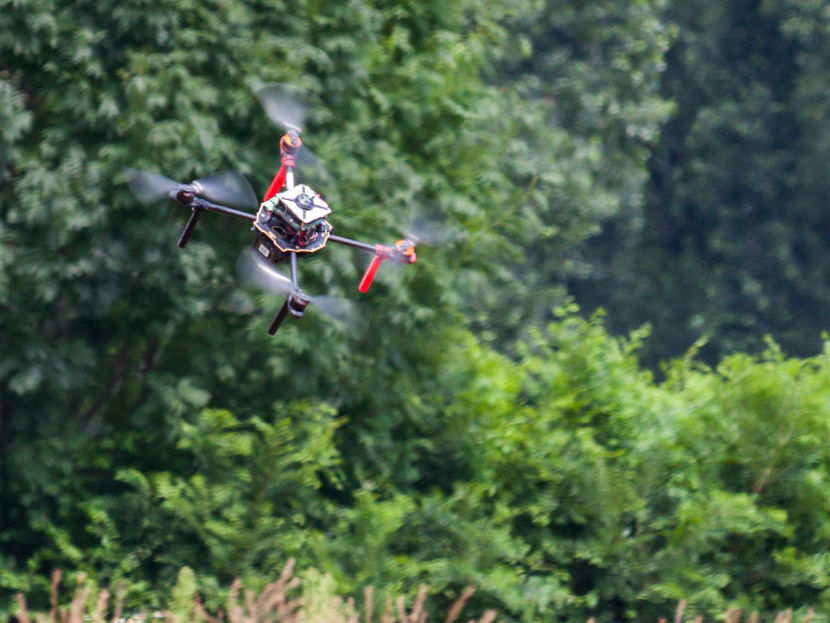
\includegraphics[width=0.235\textwidth]{./fig/photos/control_2_1-5.jpg}};
    \begin{scope}[x={(a.south east)},y={(a.north west)}]
      %%{ grid
      % % useful grid to help you find coordinates for plotting the overlay
      % \draw[black, xstep=.1, ystep=.1] (0,0) grid (1,1);
      % \foreach \i in {0,0.1,0.2,0.3,0.4,0.5,0.6,0.7,0.8,0.9,1} {
      %   \node[align=center] at (\i, -0.05) {\i};
      %   \node[align=center] at (\i, 1.05) {\i};
      %   \node[align=center] at (-0.05, \i) {\i};
      %   \node[align=center] at (1.05, \i) {\i};
      % }
      %%}
      % plot some stuff over the image
      \fill[white] (0.001, 0.001) rectangle (0.12,0.13);
      \fill[draw=black, draw opacity=0.5, fill opacity=0] (0,0) rectangle (1, 1);
      \node[imgletter,text=black] (label) at (a.south west) {(a)};
    \end{scope}
  \end{tikzpicture}}
  \hfill%
  \subfloat {\begin{tikzpicture}
    \node[anchor=south west,inner sep=0] (a) at (0,0) { 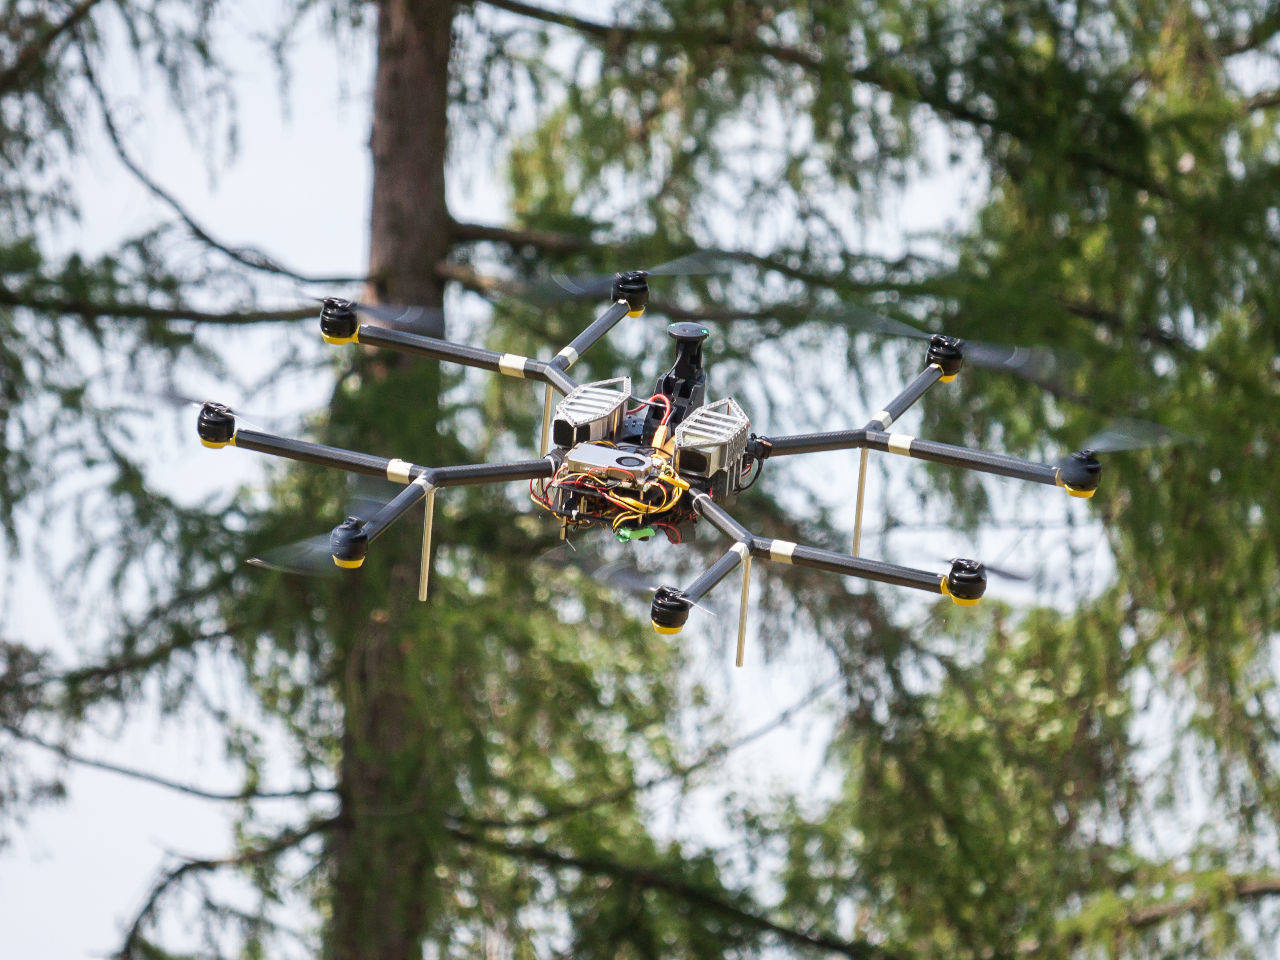
\includegraphics[width=0.235\textwidth]{./fig/photos/eagle_2_1-5.jpg}};
    \begin{scope}[x={(a.south east)},y={(a.north west)}]
      %%{ grid
      % % useful grid to help you find coordinates for plotting the overlay
      % \draw[black, xstep=.1, ystep=.1] (0,0) grid (1,1);
      % \foreach \i in {0,0.1,0.2,0.3,0.4,0.5,0.6,0.7,0.8,0.9,1} {
      %   \node[align=center] at (\i, -0.05) {\i};
      %   \node[align=center] at (\i, 1.05) {\i};
      %   \node[align=center] at (-0.05, \i) {\i};
      %   \node[align=center] at (1.05, \i) {\i};
      % }
      %%}
      % plot some stuff over the image
      \fill[white] (0.001, 0.001) rectangle (0.12,0.13);
      \fill[draw=black, draw opacity=0.5, fill opacity=0] (0,0) rectangle (1, 1);
      \node[imgletter,text=black] (label) at (a.south west) {(b)};
    \end{scope}
  \end{tikzpicture}}
  \caption{Novel control approaches can be tested on a real hardware. Off-the-shelf platforms such as (a) Tarot 650, and also (b) custom-built airframes, can be equipped with the proposed system.}
  \label{fig:control}
\end{figure}

%%}

%%}

%%{ Sec: Data gathering

\section{Data gathering}

%%{ Fig: dronument

\begin{figure}
  \centering
  \subfloat {\begin{tikzpicture}
    \node[anchor=south west,inner sep=0] (a) at (0,0) { 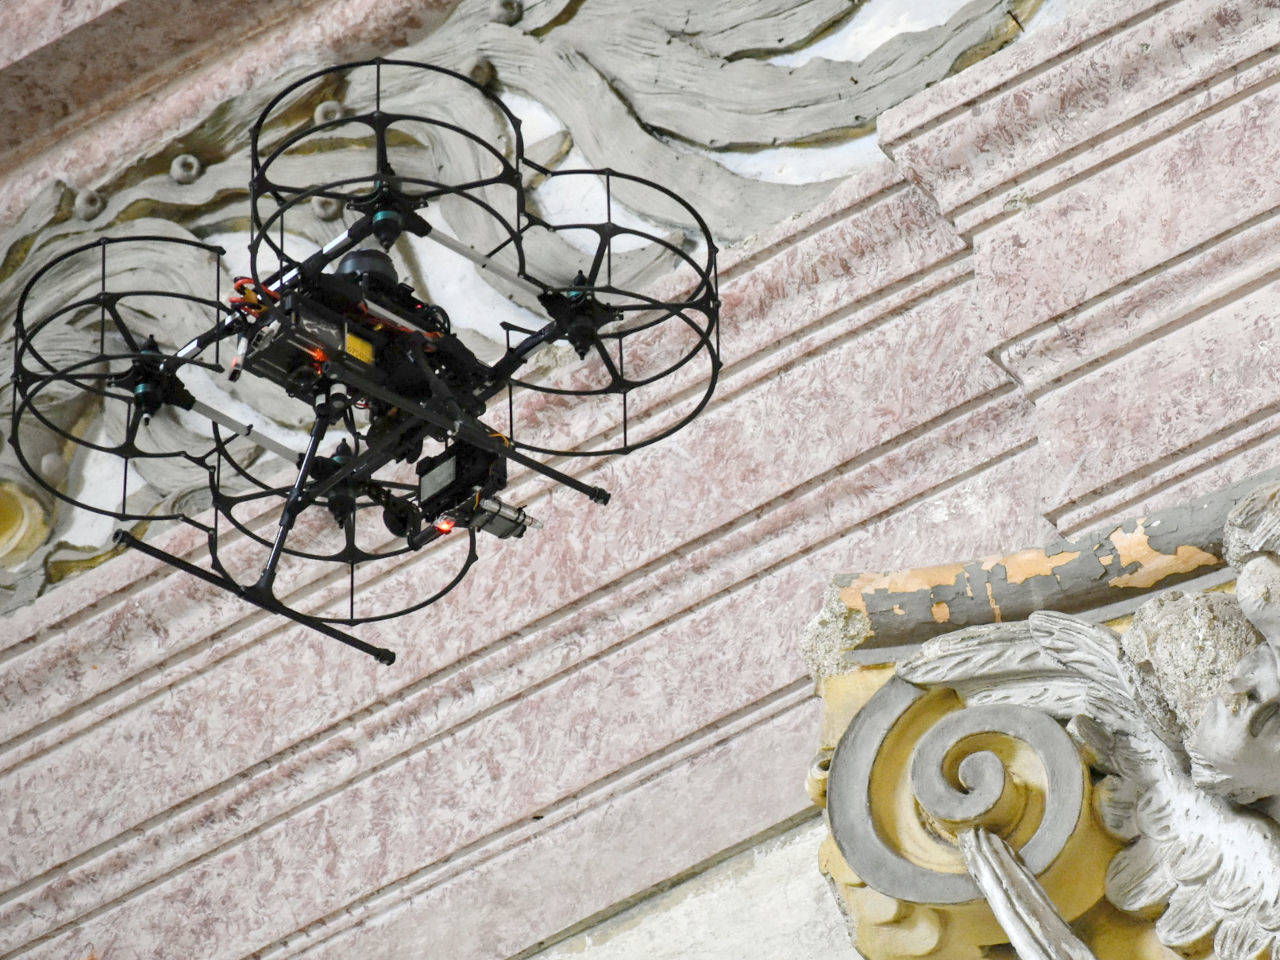
\includegraphics[width=0.235\textwidth]{./fig/photos/dronument_2_2_1-5.jpg}};
    \begin{scope}[x={(a.south east)},y={(a.north west)}]
      %%{ grid
      % % useful grid to help you find coordinates for plotting the overlay
      % \draw[black, xstep=.1, ystep=.1] (0,0) grid (1,1);
      % \foreach \i in {0,0.1,0.2,0.3,0.4,0.5,0.6,0.7,0.8,0.9,1} {
      %   \node[align=center] at (\i, -0.05) {\i};
      %   \node[align=center] at (\i, 1.05) {\i};
      %   \node[align=center] at (-0.05, \i) {\i};
      %   \node[align=center] at (1.05, \i) {\i};
      % }
      %%}
      % plot some stuff over the image
      \fill[white] (0.001, 0.001) rectangle (0.12,0.13);
      \fill[draw=black, draw opacity=0.5, fill opacity=0] (0,0) rectangle (1, 1);
      \node[imgletter,text=black] (label) at (a.south west) {(a)};
    \end{scope}
  \end{tikzpicture}}
  \hfill%
  \subfloat {\begin{tikzpicture}
    \node[anchor=south west,inner sep=0] (a) at (0,0) { 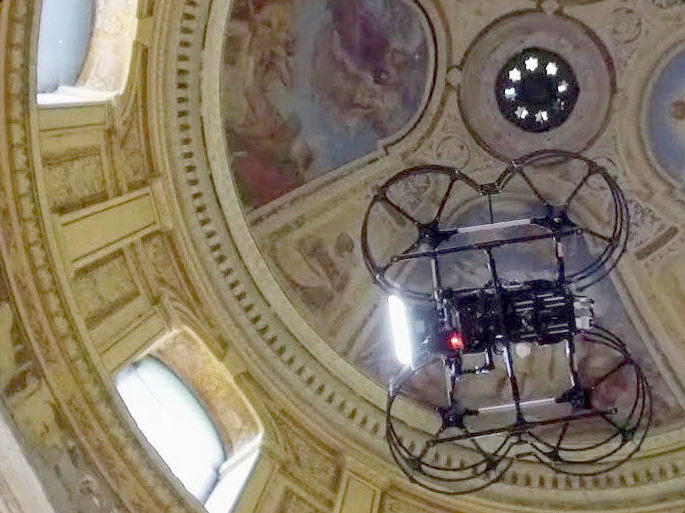
\includegraphics[width=0.235\textwidth]{./fig/photos/dronument_2_1-5.jpg}};
    \begin{scope}[x={(a.south east)},y={(a.north west)}]
      %%{ grid
      % % useful grid to help you find coordinates for plotting the overlay
      % \draw[black, xstep=.1, ystep=.1] (0,0) grid (1,1);
      % \foreach \i in {0,0.1,0.2,0.3,0.4,0.5,0.6,0.7,0.8,0.9,1} {
      %   \node[align=center] at (\i, -0.05) {\i};
      %   \node[align=center] at (\i, 1.05) {\i};
      %   \node[align=center] at (-0.05, \i) {\i};
      %   \node[align=center] at (1.05, \i) {\i};
      % }
      %%}
      % plot some stuff over the image
      \fill[white] (0.001, 0.001) rectangle (0.12,0.13);
      \fill[draw=black, draw opacity=0.5, fill opacity=0] (0,0) rectangle (1, 1);
      \node[imgletter,text=black] (label) at (a.south west) {(b)};
    \end{scope}
  \end{tikzpicture}}
  \caption{An inspection of an indoor historical building is conducted (a) to monitor the state of frescoes, and (b) to assess the state of wall paintings.}
  \label{fig:dronument}
\end{figure}

%%}

%%}

%%{ Sec: Swarms and formations

\section{UAV swarms and formations}
\label{sec:uav_swarms_and_formations}

%%{ Fig: swamrs

\begin{figure}
  \centering
  \subfloat {\begin{tikzpicture}
    \node[anchor=south west,inner sep=0] (a) at (0,0) { 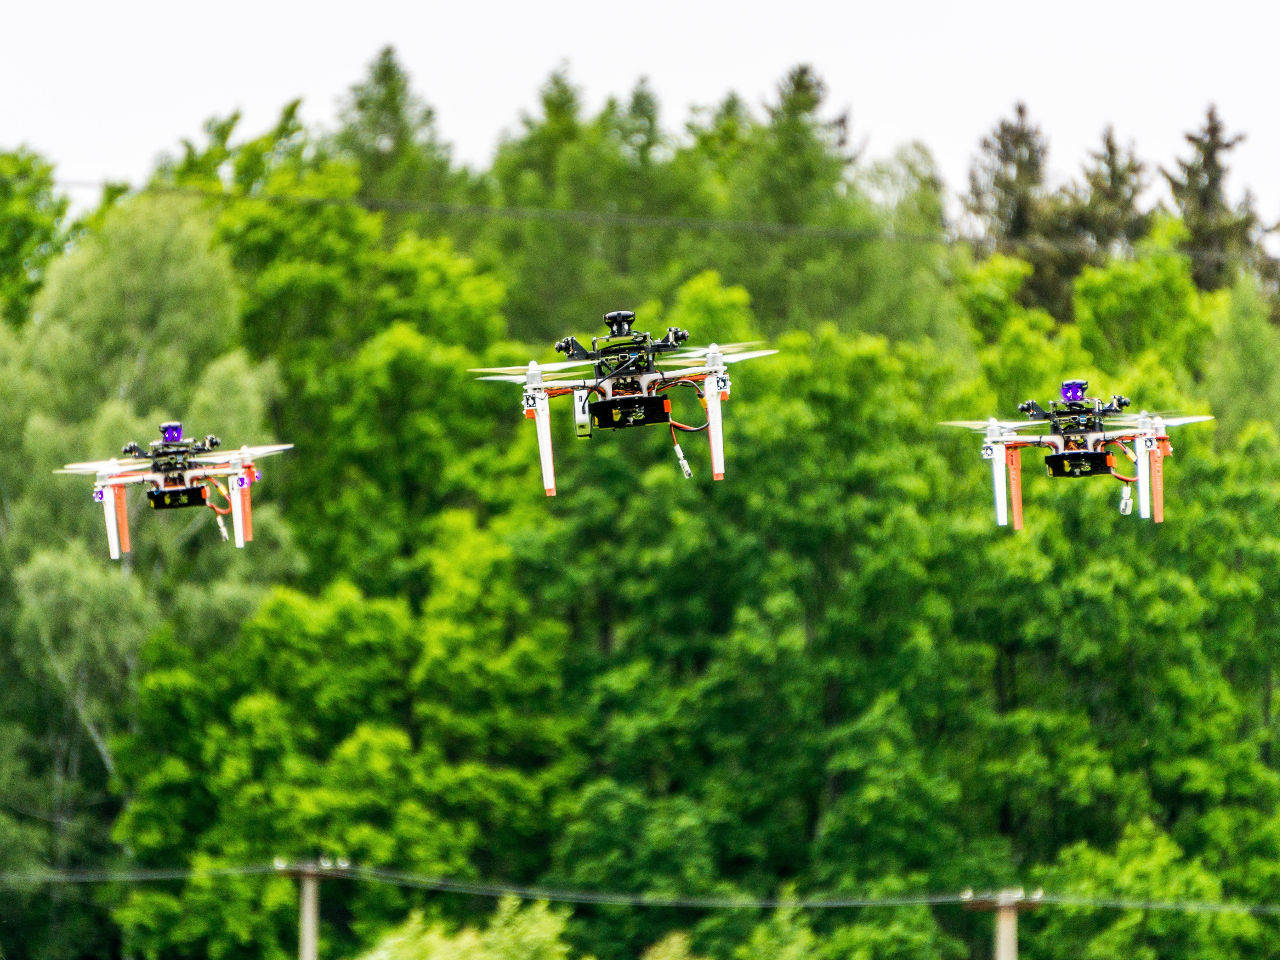
\includegraphics[width=0.235\textwidth]{./fig/photos/swarm_2_1-5.jpg}};
    \begin{scope}[x={(a.south east)},y={(a.north west)}]
      %%{ grid
      % % useful grid to help you find coordinates for plotting the overlay
      % \draw[black, xstep=.1, ystep=.1] (0,0) grid (1,1);
      % \foreach \i in {0,0.1,0.2,0.3,0.4,0.5,0.6,0.7,0.8,0.9,1} {
      %   \node[align=center] at (\i, -0.05) {\i};
      %   \node[align=center] at (\i, 1.05) {\i};
      %   \node[align=center] at (-0.05, \i) {\i};
      %   \node[align=center] at (1.05, \i) {\i};
      % }
      %%}
      \fill[white] (0.001, 0.001) rectangle (0.12,0.13);
      % plot some stuff over the image
      \fill[draw=black, draw opacity=0.5, fill opacity=0] (0,0) rectangle (1, 1);
      \node[imgletter,text=black] (label) at (a.south west) {(a)};
    \end{scope}
  \end{tikzpicture}}
  \hfill
  \subfloat {\begin{tikzpicture}
    \node[anchor=south west,inner sep=0] (a) at (0,0) { 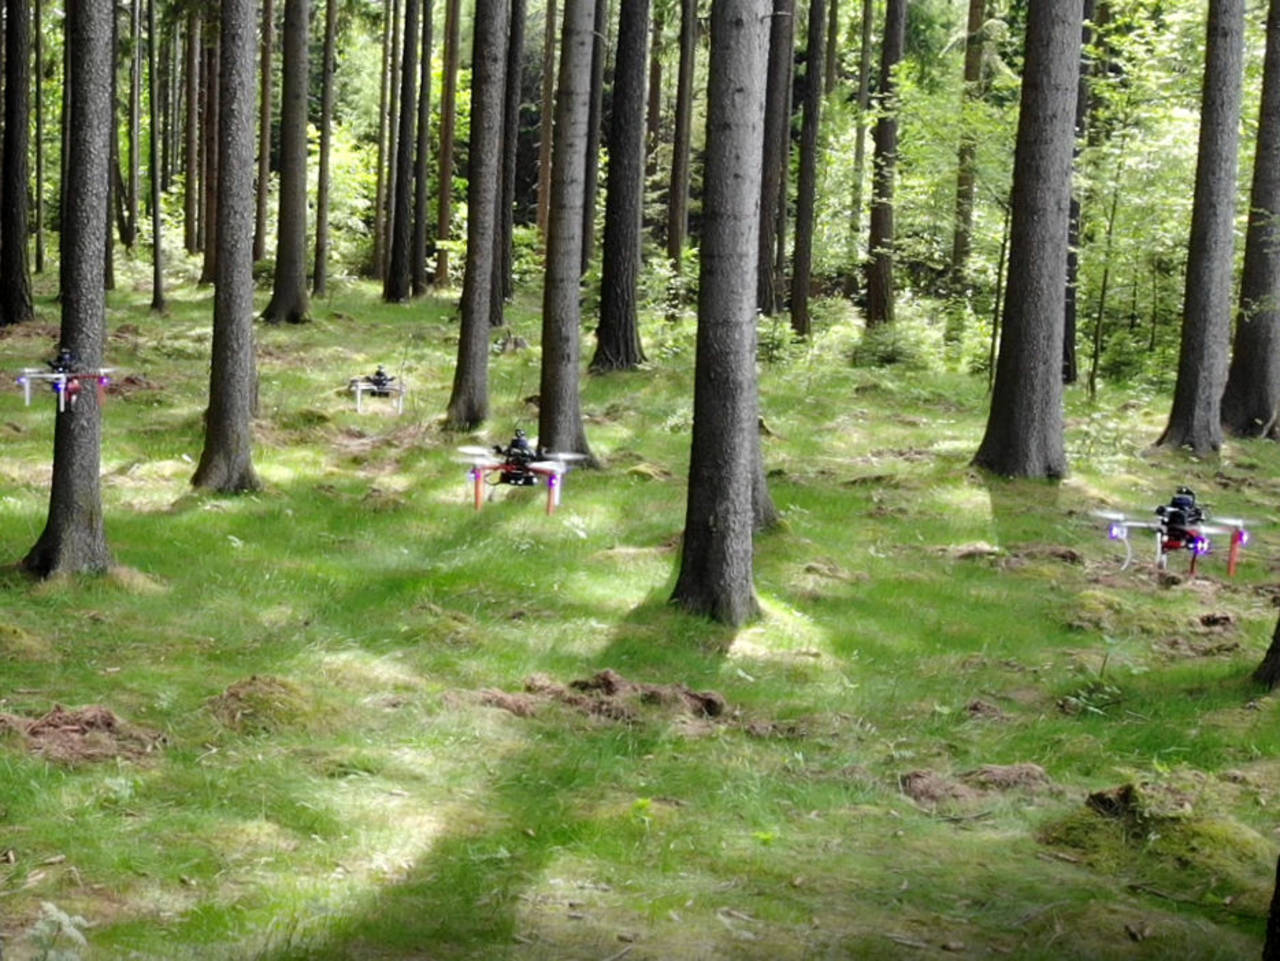
\includegraphics[width=0.235\textwidth]{./fig/photos/swarm_forest_2_1-5.jpg}};
    \begin{scope}[x={(a.south east)},y={(a.north west)}]
      %%{ grid
      % useful grid to help you find coordinates for plotting the overlay
      % \draw[black, xstep=.1, ystep=.1] (0,0) grid (1,1);
      % \foreach \i in {0,0.1,0.2,0.3,0.4,0.5,0.6,0.7,0.8,0.9,1} {
      %   \node[align=center] at (\i, -0.05) {\i};
      %   \node[align=center] at (\i, 1.05) {\i};
      %   \node[align=center] at (-0.05, \i) {\i};
      %   \node[align=center] at (1.05, \i) {\i};
      % }
      %%}

      \draw[->, white, thick] (0.45, 0.20) -- (0.07, 0.57);
      \draw[->, white, thick] (0.45, 0.20) -- (0.30, 0.55);
      \draw[->, white, thick] (0.45, 0.20) -- (0.40, 0.45);
      \draw[->, white, thick] (0.45, 0.20) -- (0.85, 0.40);
      \draw (0.45,0.15) node [text=white] {\small UAVs};

      \fill[white] (0.001, 0.001) rectangle (0.12,0.13);
      % plot some stuff over the image
      \fill[draw=black, draw opacity=0.5, fill opacity=0] (0,0) rectangle (1, 1);
      \node[imgletter,text=black] (label) at (a.south west) {(b)};
    \end{scope}
  \end{tikzpicture}}
  \caption{Swarms of multirotor \acp{UAV} testing novel flocking algorithms while localized (a) by a \ac{GNSS} system, and (b) by onboard sensors only within a forest environment.}
  \label{fig:swarms}
\end{figure}

%%}

%%}

%%{ Sec: DARPA SubT

\section{The DARPA Subterranean (SubT) challenge}

%%{ Fig: DARPA SubT

\begin{figure}
  \centering
  \subfloat {\begin{tikzpicture}
    \node[anchor=south west,inner sep=0] (a) at (0,0) { 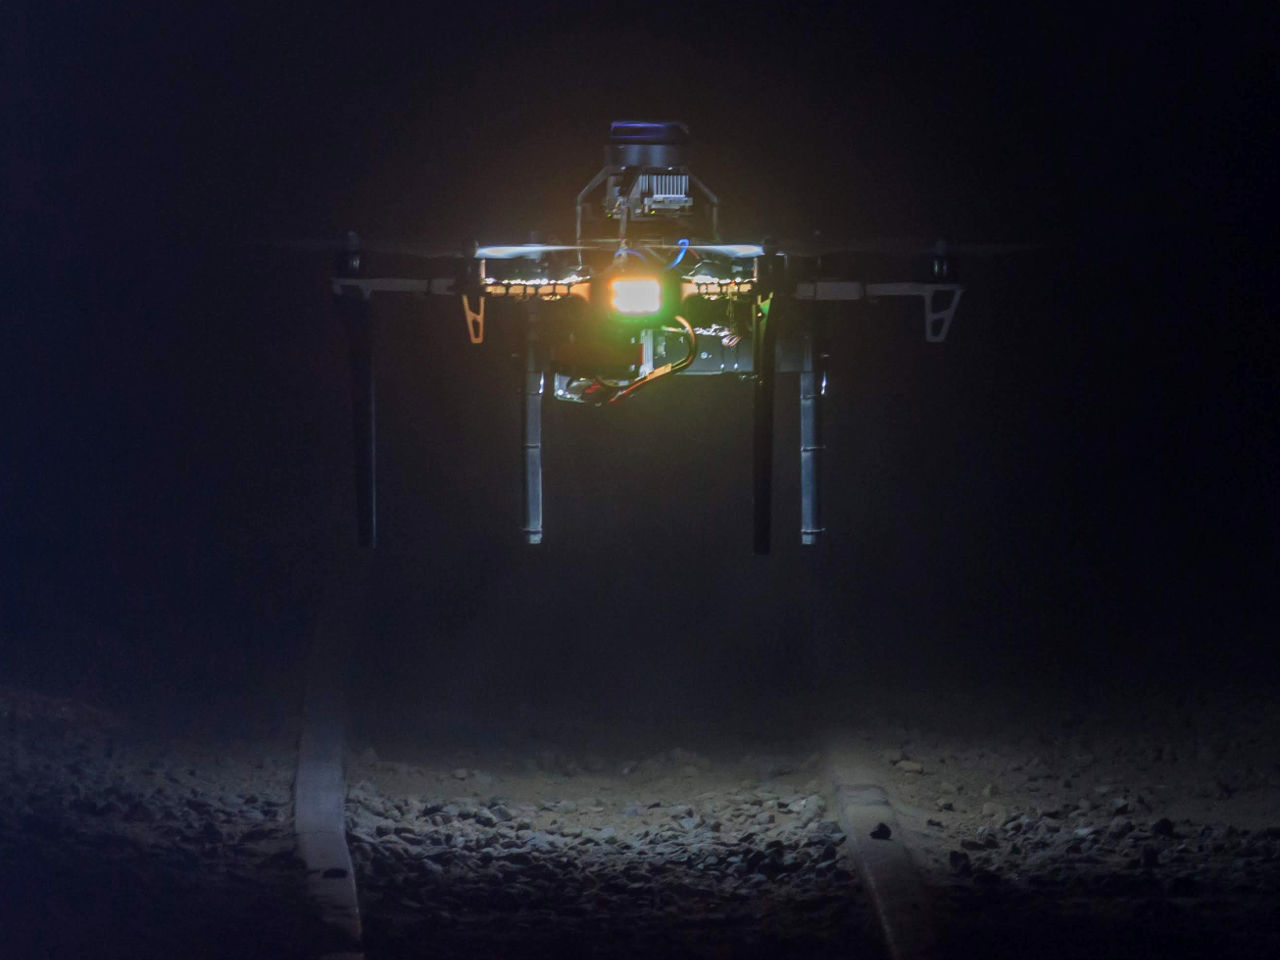
\includegraphics[width=0.235\textwidth]{./fig/photos/darpa_stix_2_1-5.jpg}};
    \begin{scope}[x={(a.south east)},y={(a.north west)}]
      %%{ grid
      % % useful grid to help you find coordinates for plotting the overlay
      % \draw[black, xstep=.1, ystep=.1] (0,0) grid (1,1);
      % \foreach \i in {0,0.1,0.2,0.3,0.4,0.5,0.6,0.7,0.8,0.9,1} {
      %   \node[align=center] at (\i, -0.05) {\i};
      %   \node[align=center] at (\i, 1.05) {\i};
      %   \node[align=center] at (-0.05, \i) {\i};
      %   \node[align=center] at (1.05, \i) {\i};
      % }
      %%}
      % plot some stuff over the image
      \fill[white] (0.001, 0.001) rectangle (0.12,0.13);
      \fill[draw=black, draw opacity=0.5, fill opacity=0] (0,0) rectangle (1, 1);
      \node[imgletter,text=black] (label) at (a.south west) {(a)};
    \end{scope}
  \end{tikzpicture}}
  \hfill%
  \subfloat {\begin{tikzpicture}
    \node[anchor=south west,inner sep=0] (a) at (0,0) { 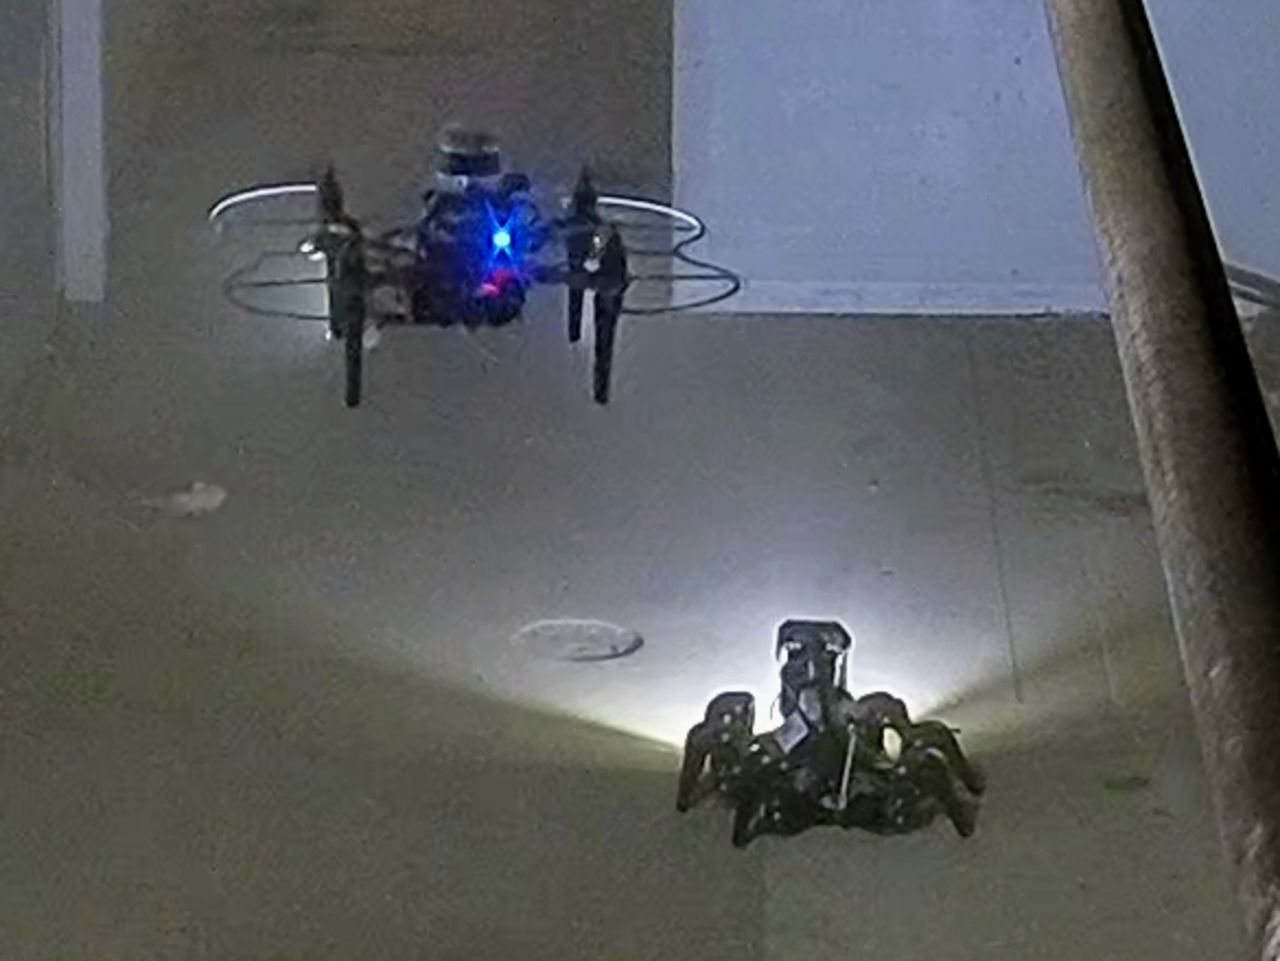
\includegraphics[width=0.235\textwidth]{./fig/photos/darpa_drone_beta_2_1-5.jpg}};
    \begin{scope}[x={(a.south east)},y={(a.north west)}]
      %%{ grid
      % % useful grid to help you find coordinates for plotting the overlay
      % \draw[black, xstep=.1, ystep=.1] (0,0) grid (1,1);
      % \foreach \i in {0,0.1,0.2,0.3,0.4,0.5,0.6,0.7,0.8,0.9,1} {
      %   \node[align=center] at (\i, -0.05) {\i};
      %   \node[align=center] at (\i, 1.05) {\i};
      %   \node[align=center] at (-0.05, \i) {\i};
      %   \node[align=center] at (1.05, \i) {\i};
      % }
      %%}
      % plot some stuff over the image
      \fill[white] (0.001, 0.001) rectangle (0.12,0.13);
      \fill[draw=black, draw opacity=0.5, fill opacity=0] (0,0) rectangle (1, 1);
      \node[imgletter,text=black] (label) at (a.south west) {(b)};
    \end{scope}
  \end{tikzpicture}}
  \caption{Unmanned Aerial Vehicles during the \ac{DARPA} SubT challenge. The photos depict (a) a \ac{UAV} exploring an underground mine, and (b) mapping an unfinished nuclear power plant.}
  \label{fig:darpa}
\end{figure}

%%}

%%}

%%{ Sec: MBZIRC 2017

\section{MBZIRC 2017 competition}

\fullciteinbox{baca2019autonomous}{}
\fullciteinbox{loianno2018localization}{}

%%{ Fig: MBZIRC 2017

\begin{figure}
  \centering
  \subfloat {\begin{tikzpicture}
    \node[anchor=south west,inner sep=0] (a) at (0,0) { 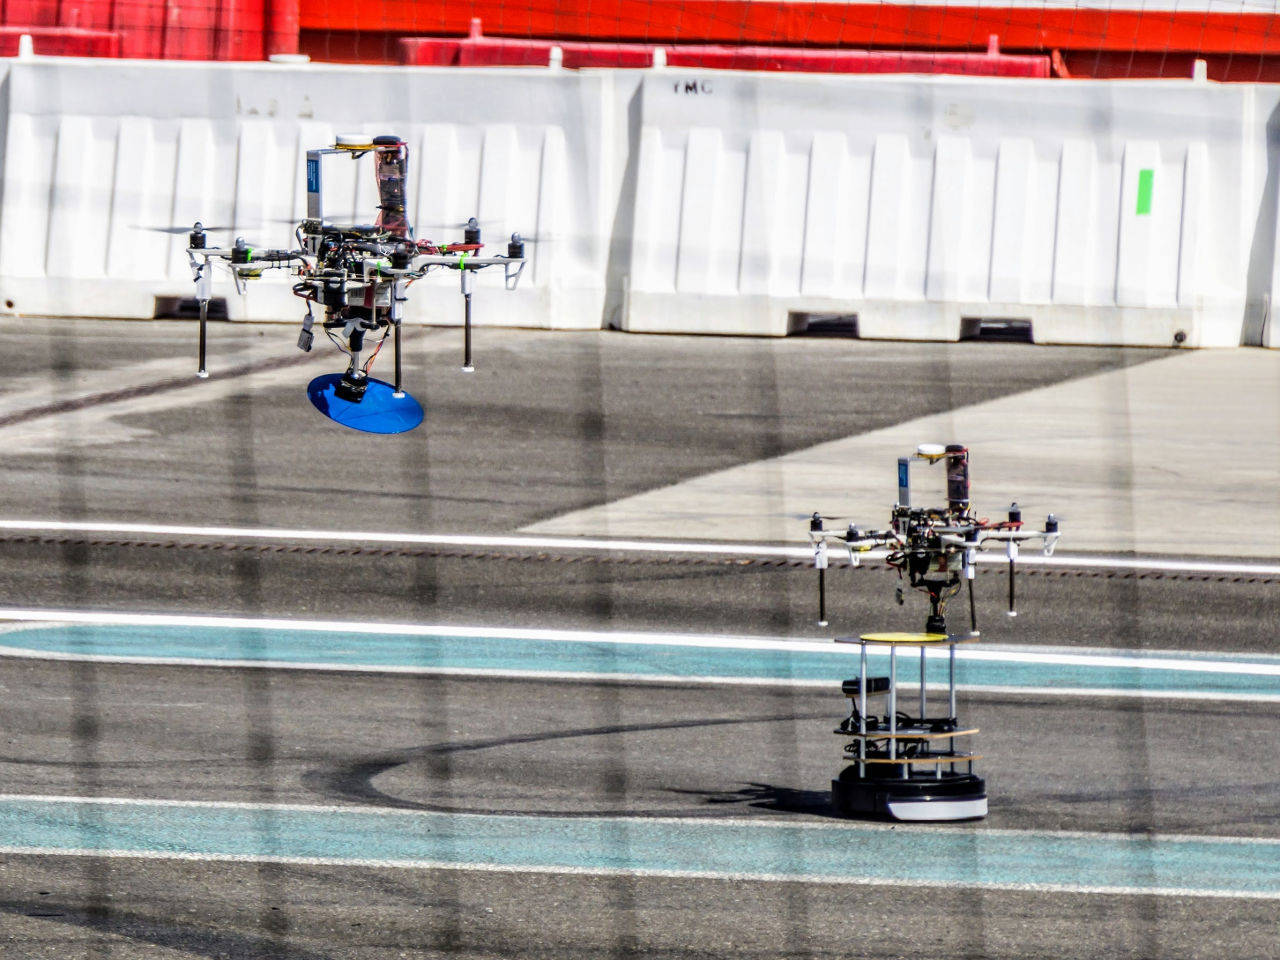
\includegraphics[width=0.235\textwidth]{./fig/photos/grasping_2017_2_1-5.jpg}};
    \begin{scope}[x={(a.south east)},y={(a.north west)}]
      %%{ grid
      % % useful grid to help you find coordinates for plotting the overlay
      % \draw[black, xstep=.1, ystep=.1] (0,0) grid (1,1);
      % \foreach \i in {0,0.1,0.2,0.3,0.4,0.5,0.6,0.7,0.8,0.9,1} {
      %   \node[align=center] at (\i, -0.05) {\i};
      %   \node[align=center] at (\i, 1.05) {\i};
      %   \node[align=center] at (-0.05, \i) {\i};
      %   \node[align=center] at (1.05, \i) {\i};
      % }
      %%}
      % plot some stuff over the image
      \fill[white] (0.001, 0.001) rectangle (0.12,0.13);
      \fill[draw=black, draw opacity=0.5, fill opacity=0] (0,0) rectangle (1, 1);
      \node[imgletter,text=black] (label) at (a.south west) {(a)};
    \end{scope}
  \end{tikzpicture}}
  \hfill%
  \subfloat {\begin{tikzpicture}
    \node[anchor=south west,inner sep=0] (a) at (0,0) { 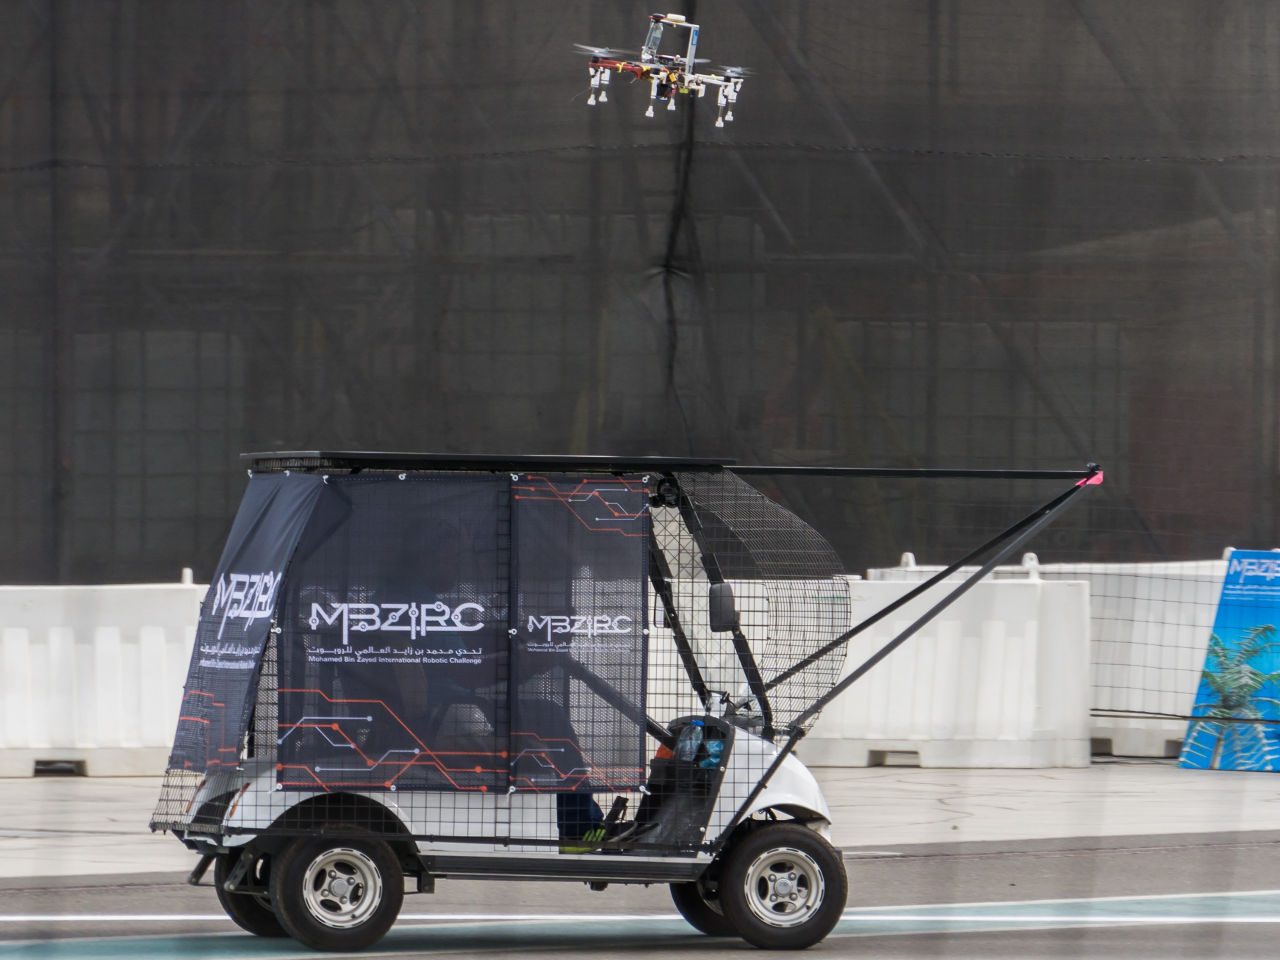
\includegraphics[width=0.235\textwidth]{./fig/photos/landing_2017_2_1-5.jpg}};
    \begin{scope}[x={(a.south east)},y={(a.north west)}]
      %%{ grid
      % % useful grid to help you find coordinates for plotting the overlay
      % \draw[black, xstep=.1, ystep=.1] (0,0) grid (1,1);
      % \foreach \i in {0,0.1,0.2,0.3,0.4,0.5,0.6,0.7,0.8,0.9,1} {
      %   \node[align=center] at (\i, -0.05) {\i};
      %   \node[align=center] at (\i, 1.05) {\i};
      %   \node[align=center] at (-0.05, \i) {\i};
      %   \node[align=center] at (1.05, \i) {\i};
      % }
      %%}
      % plot some stuff over the image
      \fill[white] (0.001, 0.001) rectangle (0.12,0.13);
      \fill[draw=black, draw opacity=0.5, fill opacity=0] (0,0) rectangle (1, 1);
      \node[imgletter,text=black] (label) at (a.south west) {(b)};
    \end{scope}
  \end{tikzpicture}}
  \caption{The CTU-UPENN-UoL team during the MBZIRC 2017 competition. The photos show (a) two \acp{UAV} while delivering ferrous objects, and (b) a \ac{UAV} during autonomous landing on a moving car.}
  \label{fig:mbzirc_2017}
\end{figure}

%%}

%%}

%%{ Sec: MBZIRC 2020

\section{MBZIRC 2020 competition}

%%{ Fig: MBZIRC 2020

\begin{figure}
  \centering
  \subfloat {\begin{tikzpicture}
    \node[anchor=south west,inner sep=0] (a) at (0,0) { 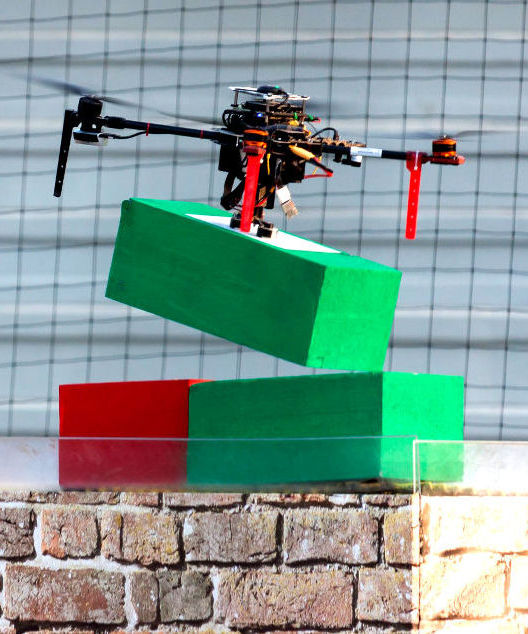
\includegraphics[width=0.155\textwidth]{./fig/photos/brick_placing_1-25_1-5.jpg}};
    \begin{scope}[x={(a.south east)},y={(a.north west)}]
      %%{ grid
      % % useful grid to help you find coordinates for plotting the overlay
      % \draw[black, xstep=.1, ystep=.1] (0,0) grid (1,1);
      % \foreach \i in {0,0.1,0.2,0.3,0.4,0.5,0.6,0.7,0.8,0.9,1} {
      %   \node[align=center] at (\i, -0.05) {\i};
      %   \node[align=center] at (\i, 1.05) {\i};
      %   \node[align=center] at (-0.05, \i) {\i};
      %   \node[align=center] at (1.05, \i) {\i};
      % }
      %%}
      % plot some stuff over the image
      \fill[white] (0.001, 0.001) rectangle (0.18,0.13);
      \fill[draw=black, draw opacity=0.5, fill opacity=0] (0,0) rectangle (1, 1);
      \node[imgletter,text=black] (label) at (a.south west) {(a)};
    \end{scope}
  \end{tikzpicture}}
  \hfill%
  \subfloat {\begin{tikzpicture}
    \node[anchor=south west,inner sep=0] (a) at (0,0) { 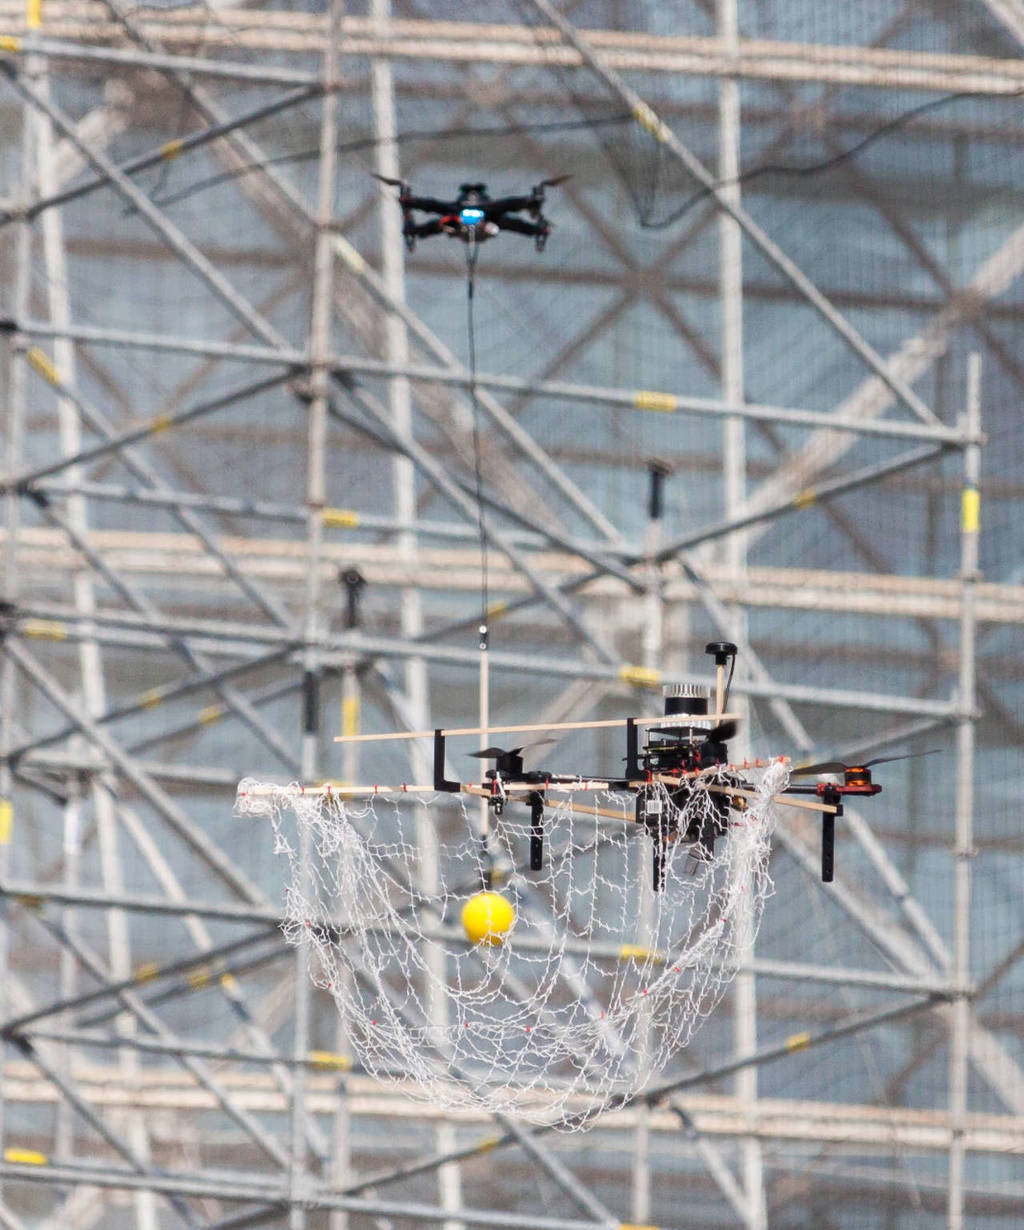
\includegraphics[width=0.155\textwidth]{./fig/photos/ball_catching_1-25_1-5.jpg}};
    \begin{scope}[x={(a.south east)},y={(a.north west)}]
      %%{ grid
      % % useful grid to help you find coordinates for plotting the overlay
      % \draw[black, xstep=.1, ystep=.1] (0,0) grid (1,1);
      % \foreach \i in {0,0.1,0.2,0.3,0.4,0.5,0.6,0.7,0.8,0.9,1} {
      %   \node[align=center] at (\i, -0.05) {\i};
      %   \node[align=center] at (\i, 1.05) {\i};
      %   \node[align=center] at (-0.05, \i) {\i};
      %   \node[align=center] at (1.05, \i) {\i};
      % }
      %%}
      % plot some stuff over the image
      \fill[white] (0.001, 0.001) rectangle (0.18,0.13);
      \fill[draw=black, draw opacity=0.5, fill opacity=0] (0,0) rectangle (1, 1);
      \node[imgletter,text=black] (label) at (a.south west) {(b)};
    \end{scope}
  \end{tikzpicture}}
  \hfill%
  \subfloat {\begin{tikzpicture}
    \node[anchor=south west,inner sep=0] (a) at (0,0) { 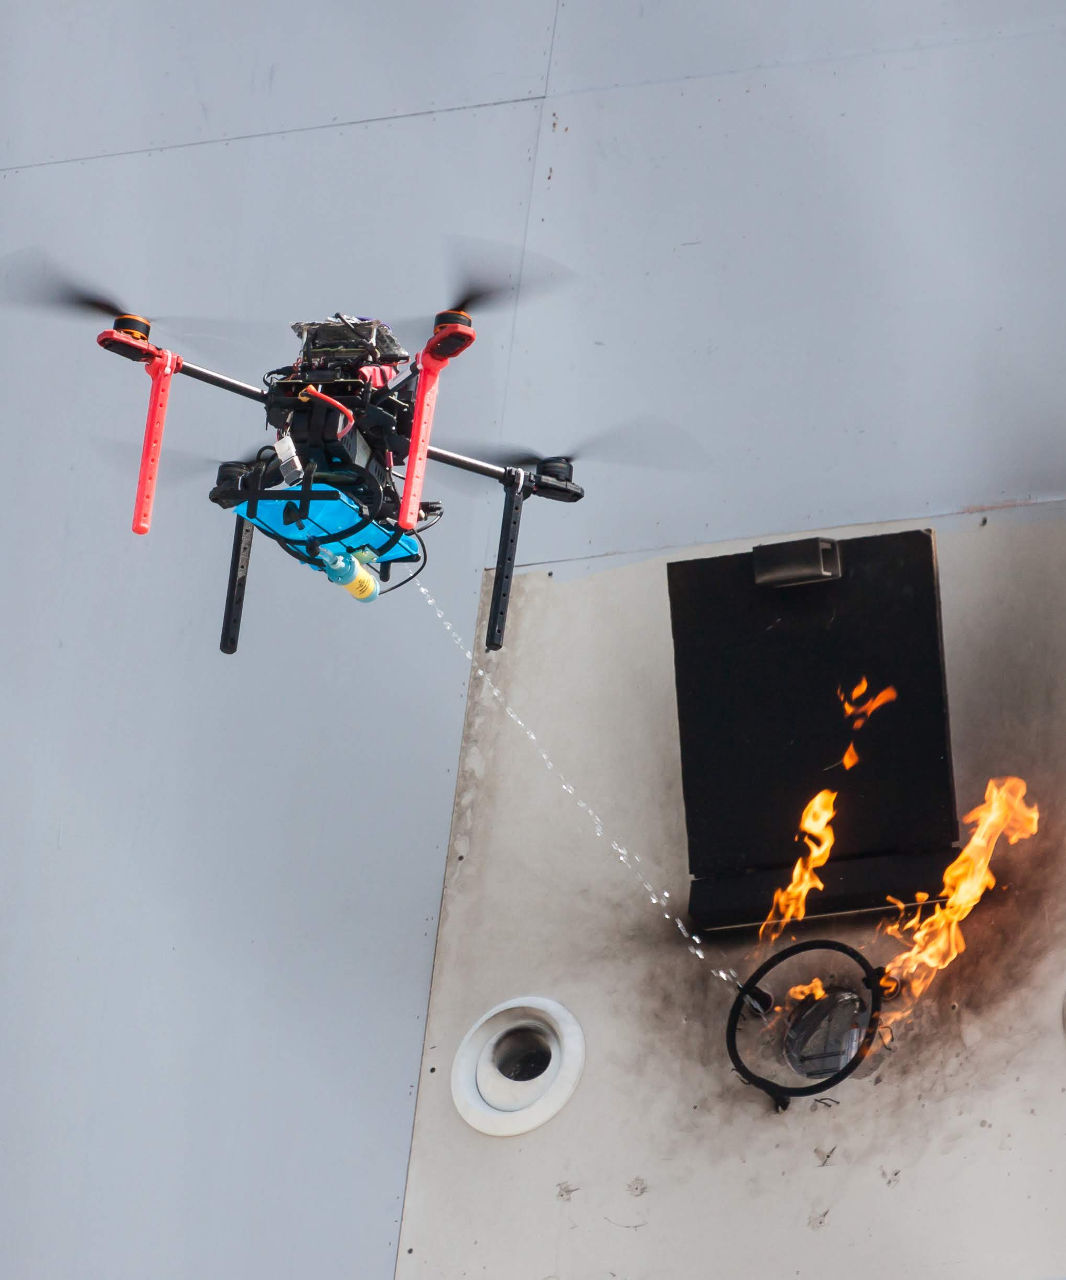
\includegraphics[width=0.155\textwidth]{./fig/photos/ext_1-25_1-5.jpg}};
    \begin{scope}[x={(a.south east)},y={(a.north west)}]
      %%{ grid
      % % useful grid to help you find coordinates for plotting the overlay
      % \draw[black, xstep=.1, ystep=.1] (0,0) grid (1,1);
      % \foreach \i in {0,0.1,0.2,0.3,0.4,0.5,0.6,0.7,0.8,0.9,1} {
      %   \node[align=center] at (\i, -0.05) {\i};
      %   \node[align=center] at (\i, 1.05) {\i};
      %   \node[align=center] at (-0.05, \i) {\i};
      %   \node[align=center] at (1.05, \i) {\i};
      % }
      %%}
      % plot some stuff over the image
      \fill[white] (0.001, 0.001) rectangle (0.18,0.13);
      \fill[draw=black, draw opacity=0.5, fill opacity=0] (0,0) rectangle (1, 1);
      \node[imgletter,text=black] (label) at (a.south west) {(c)};
    \end{scope}
  \end{tikzpicture}}\\
  \vspace{-0.8em}
  \subfloat {\begin{tikzpicture}
    \node[anchor=south west,inner sep=0] (a) at (0,0) { 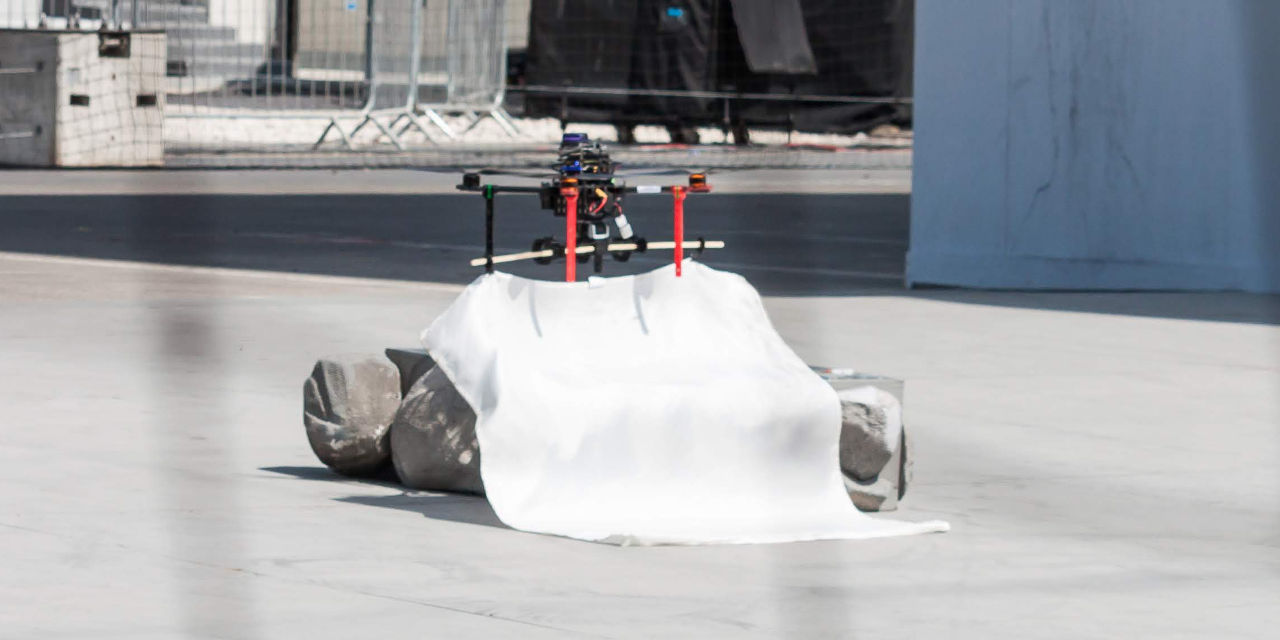
\includegraphics[width=0.235\textwidth]{./fig/photos/blanket_2_1.jpg}};
    \begin{scope}[x={(a.south east)},y={(a.north west)}]
      %%{ grid
      % % useful grid to help you find coordinates for plotting the overlay
      % \draw[black, xstep=.1, ystep=.1] (0,0) grid (1,1);
      % \foreach \i in {0,0.1,0.2,0.3,0.4,0.5,0.6,0.7,0.8,0.9,1} {
      %   \node[align=center] at (\i, -0.05) {\i};
      %   \node[align=center] at (\i, 1.05) {\i};
      %   \node[align=center] at (-0.05, \i) {\i};
      %   \node[align=center] at (1.05, \i) {\i};
      % }
      %%}
      % plot some stuff over the image
      \fill[white] (0.001, 0.001) rectangle (0.13,0.20);
      \fill[draw=black, draw opacity=0.5, fill opacity=0] (0,0) rectangle (1, 1);
      \node[imgletter,text=black] (label) at (a.south west) {(d)};
    \end{scope}
  \end{tikzpicture}}
  \hfill%
  \subfloat {\begin{tikzpicture}
    \node[anchor=south west,inner sep=0] (a) at (0,0) { 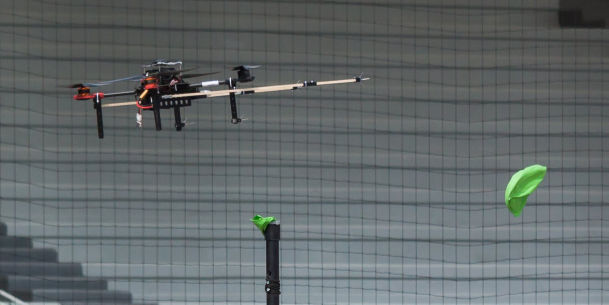
\includegraphics[width=0.235\textwidth]{./fig/photos/popping_2_1.jpg}};
    \begin{scope}[x={(a.south east)},y={(a.north west)}]
      %%{ grid
      % % useful grid to help you find coordinates for plotting the overlay
      % \draw[black, xstep=.1, ystep=.1] (0,0) grid (1,1);
      % \foreach \i in {0,0.1,0.2,0.3,0.4,0.5,0.6,0.7,0.8,0.9,1} {
      %   \node[align=center] at (\i, -0.05) {\i};
      %   \node[align=center] at (\i, 1.05) {\i};
      %   \node[align=center] at (-0.05, \i) {\i};
      %   \node[align=center] at (1.05, \i) {\i};
      % }
      %%}
      % plot some stuff over the image
      \fill[white] (0.001, 0.001) rectangle (0.13,0.20);
      \fill[draw=black, draw opacity=0.5, fill opacity=0] (0,0) rectangle (1, 1);
      \node[imgletter,text=black] (label) at (a.south west) {(e)};
    \end{scope}
  \end{tikzpicture}}
  \caption{The CTU-UPENN-NYU team during the MBZIRC 2020 competition. The photos depict (a) autonomous wall building, (b) autonomous ball catching, (c) autonomous fire extinguishing, (d) autonomous fire blanket deployment, and (e) autonomous balloon popping.}
  \label{fig:mbzirc_2020}
\end{figure}

%%}

%%}

% INCLUDE THE FOLLOWING PDFS
\includepaper{loianno2018localization}
\includepaper{baca2019autonomous}

%%}

%% | ------------------------ Chapter 5 ----------------------- |

%%{ Ionizing Radiation Detection and Localization by UAVs

\chapternoclear{Ionizing Radiation Detection and Localization by UAVs}
\chaptermark{Ionizing Radiation Sources Localization}

Ongoing research realized in the accepted TACR 2020-2022 project FW01010317:\\
``\textit{Lokalizace zdrojů ionizující radiace pomocí malých bezpilotních helikoptér s detektorem na principu Comptonovy kamery}''.

Relevant author's publications (will be discussed):
\fullciteinbox{baca2016miniaturized}{}
\fullciteinbox{baca2018rospix}{}
\fullciteinbox{baca2018timepix}{}
\fullciteinbox{baca2019timepix}{}
\fullciteinbox{stibinger2020localization}{}

% INCLUDE THE FOLLOWING PDFs
\includepaper{baca2018timepix}
\includepaper{baca2019timepix}
\includepaper{stibinger2020localization}

%%}

%%}

%% | ------------------------ Chapter 6 ----------------------- |

%%{ Conclusion

\chapternoclear{Conclusion}

\todo{}

%%}

%% | ----------------------- References ----------------------- |

%%{ References

\appendix
\renewcommand\chaptername{Appendix}

\chapternoclear{References}

Below are listed all publications of the author.
Each citation is displayed with percentage contribution of the author and number of citations based on Web of Science~(WoS), Scopus and Google Scholar~(GS).
\todo{updated citations}

%%{ Core publications

\section{Thesis core publications}

\subsection*{Core articles in peer-reviewed journals}
\printbibliography[keyword={mine},keyword={phd_related},keyword={journal},keyword={core},notkeyword={submitted},heading=none,title={}]

\subsection*{Core conference proceedings}
\printbibliography[keyword={mine},keyword={phd_related},keyword={conference},keyword={core},notkeyword={submitted},heading=none,title={}]

\subsection*{Core articles --- submitted}
\printbibliography[keyword={mine},keyword={phd_related},keyword={submitted},keyword={core},heading=none,title={}]

%%}

%%{ Related publications

\section{Thesis-related author's publications}

\subsection*{Thesis-related articles in peer-reviewed journals}
\printbibliography[keyword={mine},keyword={phd_related},keyword={journal},notkeyword={core},notkeyword={submitted},heading=none,title={}]

% \subsection*{Thesis-related articles in peer-reviewed journals only with CiteScore~(CS)}
% \printbibliography[keyword={mine},keyword={phd_related},keyword={journal},keyword={cs},heading=none,title={}]

\subsection*{Thesis-related conference proceedings}
\printbibliography[keyword={mine},keyword={phd_related},keyword={conference},notkeyword={core},notkeyword={submitted},heading=none,title={}]

\subsection*{Thesis-related publications --- submitted}
\printbibliography[keyword={mine},keyword={phd_related},keyword={submitted},notkeyword={core},heading=none,title={}]

%%}

%%{ Partially-related publications

\section{Partially-related author's publications}

\subsection*{Partially-related articles in peer-reviewed journals}
\printbibliography[keyword={mine},keyword={phd_unrelated},keyword={journal},notkeyword={core},notkeyword={submitted},heading=none,title={}]

\subsection*{Partially-related conference proceedings}
\printbibliography[keyword={mine},keyword={phd_unrelated},keyword={conference},notkeyword={core},notkeyword={submitted},heading=none,title={}]

\subsection*{Partially-related publications --- submitted}
\printbibliography[keyword={mine},keyword={phd_unrelated},keyword={submitted},heading=none,title={}]

%%}

%%{ Cited references

\section{Cited references}
\printbibliography[notkeyword=mine,heading=none,title={}]

%%}

%%}

%% | ------------------------ Apendices ----------------------- |

%%{ Apendices

\appendix
\renewcommand\chaptername{Citations of author's publications}

\chapternoclear{Citations of author's publications}

Below are listed all citations of author's publications without self-citations.

\DeclareCiteCommand{\fullcite}
{\usebibmacro{prenote}}
{\clearfield{addendum}%
  \usedriver
  {\defcounter{minnames}{6}%
  \defcounter{maxnames}{6}}
{\thefield{entrytype}}}
{\multicitedelim}
{\usebibmacro{postnote}}

\noindent
\fullcite{saska2017system}
\begin{refsection}[citations/no_autocit/saska2017system.bib]
  \nocite{*}
  \printbibliography[heading=none,title={},env=favoritebib]
\end{refsection}

% \noindent
% \fullcite{faigl2017onsolution}
% \begin{refsection}[citations/no_autocit/faigl2017onsolution.bib]
%   \nocite{*}
%   \printbibliography[heading=none,title={},env=favoritebib]
% \end{refsection}

% \noindent
% \fullcite{saska2016formations}
% \begin{refsection}[citations/no_autocit/saska2016formations.bib]
%   \nocite{*}
%   \printbibliography[heading=none,title={},env=favoritebib]
% \end{refsection}

\noindent
\fullcite{baca2016miniaturized}
\begin{refsection}[citations/no_autocit/baca2016miniaturized.bib]
  \nocite{*}
  \printbibliography[heading=none,title={},env=favoritebib]
\end{refsection}

\noindent
\fullcite{loianno2018localization}
\begin{refsection}[citations/no_autocit/loianno2018localization.bib]
  \nocite{*}
  \printbibliography[heading=none,title={},env=favoritebib]
\end{refsection}

\noindent
\fullcite{spurny2019cooperative}
\begin{refsection}[citations/no_autocit/spurny2019cooperative.bib]
  \nocite{*}
  \printbibliography[heading=none,title={},env=favoritebib]
\end{refsection}

\noindent
\fullcite{daniel2016terrestrial}
\begin{refsection}[citations/no_autocit/daniel2016terrestrial.bib]
  \nocite{*}
  \printbibliography[heading=none,title={},env=favoritebib]
\end{refsection}

\noindent
\fullcite{baca2017autonomous}
\begin{refsection}[citations/no_autocit/baca2017autonomous.bib]
  \nocite{*}
  \printbibliography[heading=none,title={},env=favoritebib]
\end{refsection}

\noindent
\fullcite{baca2018model}
\begin{refsection}[citations/no_autocit/baca2018model.bib]
  \nocite{*}
  \printbibliography[heading=none,title={},env=favoritebib]
\end{refsection}

\noindent
\fullcite{daniel2017xray}
\begin{refsection}[citations/no_autocit/daniel2017xray.bib]
  \nocite{*}
  \printbibliography[heading=none,title={},env=favoritebib]
\end{refsection}

\noindent
\fullcite{urban2017vzlusat}
\begin{refsection}[citations/no_autocit/urban2017vzlusat.bib]
  \nocite{*}
  \printbibliography[heading=none,title={},env=favoritebib]
\end{refsection}

\noindent
\fullcite{baca2016embedded}
\begin{refsection}[citations/no_autocit/baca2016embedded.bib]
  \nocite{*}
  \printbibliography[heading=none,title={},env=favoritebib]
\end{refsection}

\noindent
\fullcite{baca2019autonomous}
\begin{refsection}[citations/no_autocit/baca2019autonomous.bib]
  \nocite{*}
  \printbibliography[heading=none,title={},env=favoritebib]
\end{refsection}

\noindent
\fullcite{saska2017documentation}
\begin{refsection}[citations/no_autocit/saska2017documentation.bib]
\nocite{*}
\printbibliography[heading=none,title={},env=favoritebib]
\end{refsection}

\noindent
\fullcite{giernacki2019realtime}
\begin{refsection}[citations/no_autocit/giernacki2019realtime.bib]
  \nocite{*}
  \printbibliography[heading=none,title={},env=favoritebib]
\end{refsection}

\noindent
\fullcite{chudoba2014localization}
\begin{refsection}[citations/no_autocit/chudoba2014localization.bib]
  \nocite{*}
  \printbibliography[heading=none,title={},env=favoritebib]
\end{refsection}

\noindent
\fullcite{saikin2020wildfire}
\begin{refsection}[citations/no_autocit/saikin2020wildfire.bib]
  \nocite{*}
  \printbibliography[heading=none,title={},env=favoritebib]
\end{refsection}

\noindent
\fullcite{daniel2019inorbit}
\begin{refsection}[citations/no_autocit/daniel2019inorbit.bib]
  \nocite{*}
  \printbibliography[heading=none,title={},env=favoritebib]
\end{refsection}

\noindent
\fullcite{baca2018timepix}
\begin{refsection}[citations/no_autocit/baca2018timepix.bib]
  \nocite{*}
  \printbibliography[heading=none,title={},env=favoritebib]
\end{refsection}

\noindent
\fullcite{baca2018rospix}
\begin{refsection}[citations/no_autocit/baca2018rospix.bib]
  \nocite{*}
  \printbibliography[heading=none,title={},env=favoritebib]
\end{refsection}

\noindent
\fullcite{spurny2016complex}
\begin{refsection}[citations/no_autocit/spurny2016complex.bib]
  \nocite{*}
  \printbibliography[heading=none,title={},env=favoritebib]
\end{refsection}

\noindent
\fullcite{chudoba2016exploration}
\begin{refsection}[citations/no_autocit/chudoba2016exploration.bib]
  \nocite{*}
  \printbibliography[heading=none,title={},env=favoritebib]
\end{refsection}

%%}

\end{document}
